\documentclass[12pt]{article}

\usepackage[margin=1in]{geometry}
\usepackage{amsmath}
\usepackage{natbib}
\usepackage[hidelinks]{hyperref}
\usepackage{array}
\usepackage{booktabs}
\usepackage{longtable}
\usepackage{graphicx}
\usepackage{xcolor}

\linespread{1.3}
\setlength{\emergencystretch}{2em}

\title{Measuring Official Exit: Labeling the Institutional Fate of China's Local Government Financing Vehicles}
\author{Shunyu Hao}
\date{\today}

\begin{document}

\maketitle

\begin{abstract}
Official reductions in China's local government financing vehicles do not show
whether the fiscal function attached to a platform disappeared, remained with
the same issuer, or moved elsewhere. This paper develops a case-level measure
of that institutional fate. A documented formal event is paired with
post-event evidence on financing, public projects, liabilities, and state-asset
control, and each case is classified as substantive exit, nominal exit,
functional transfer, or liquidation. The current working-reference file contains
ninety-four source-packet-reviewed city-platform cases awaiting independent
human confirmation: two substantive exits,
eighty-two nominal exits, ten functional transfers, and no liquidations. Every
cited evidence identifier resolves against the project inventories, and
ninety-three cases have complete local copies of their cited documents. A
separate LLM screen covers 361 candidate disclosures and produces 203
one-sided nominal-exit surrogate labels. Its sixty-one post-hoc overlap issuers
all match the reference label, but this selected overlap does not identify
population precision, recall, or four-category error. I use the measure in an
exploratory application to historical elite density. The simple association
with movement away from nominal exit is positive among eighty-four matched
cases, but adjusted estimates are sparse and unstable. The paper's contribution
is therefore a source-auditable measurement framework for distinguishing formal
compliance from functional fiscal change, not a settled causal estimate of
historical state capacity.
\end{abstract}

\section{Introduction}

China's local government financing vehicle (LGFV) exit reform poses a
measurement problem before it poses an explanation problem. Official reports
record reductions in platform counts, financing balances, and local government
debt exposure, but those figures do not reveal what happened to the government
financing and public-project functions that made the platforms important.
Official exit is not institutional exit. The same compliance statement can
describe a firm that stopped quasi-fiscal financing, a firm that continued the
same function under new language, or a reorganization that moved the function
to another local state-owned entity.

This paper measures the institutional fate of official exit. The coding rule
begins with a documented formal event and then traces the post-event location
of financing, construction, land development, liabilities, fiscal support, and
state-asset control. It assigns one of four mutually exclusive outcomes.
Substantive exit means that the issuer no longer performs the relevant
government financing function. Nominal exit means that formal compliance
language appears while the same issuer continues that function. Functional
transfer means that the original issuer exits or is reorganized while the
function moves to another local state-owned entity. Liquidation records legal
termination and remains separate because termination alone does not establish
where the fiscal function went.

The framework adapts established concerns about organizational decoupling and
LGFV transformation to a source-auditable case measure. Prior work already
shows that formal policy can diverge from organizational practice, that list
exit can coexist with continued borrowing, and that platform transformation can
change organizational form without eliminating fiscal functions
\citep{bromley_powell_2012_decoupling,zhelyazkova_kaya_schrama_2016_compliance,
fang_lu_2024_classified_regulation,li_feng_hao_2022_lgfp_transformation,
feng_wu_zhang_2022_jiaxing}. The contribution here is not the general
formal-substantive distinction. It is the joint evidence design: verify the
formal event, trace the function after that event, assign a four-category fate,
and retain the source packet and alternative interpretation for review.

The current working-reference file contains ninety-four city-platform cases
assigned through Codex source-packet review on behalf of the project author.
They await independent human confirmation. The file records two substantive
exits, eighty-two nominal exits, ten
functional transfers, and no liquidation cases. These frequencies are not
national prevalence estimates because the cases were assembled to develop and
stress-test the measure. They nevertheless establish the empirical puzzle.
Identical no-government-financing language appears in cases where former
projects moved into fiscal channels, cases where the same issuer retained
public-project and fiscal-support functions, and cases where those functions
moved through a reorganized municipal platform system. All evidence identifiers
cited by the reference labels resolve against the document and source
inventories; ninety-three cases have complete local copies of the cited
documents, and every case has a recovery URL for each cited document.

I use the new outcome in an exploratory application to historically rooted
local capacity. LGFV exit can require three contemporary processes: fiscal
absorption of eligible obligations, bureaucratic coordination of assignments
and transfers, and project or state-asset governance after reorganization.
These processes are observable in budgets, debt registers, cross-agency
decisions, transfer records, contracts, and project-level control. Historical
elite density may be associated with the institutional environments that
support them, but it is not a direct measure of any one process and also
captures education and social capital \citep{chen_kung_ma_2020_keju}. The paper
therefore treats historical capacity as an explanatory application rather than
as part of the measurement contribution.

Among the eighty-four reference cases matched to Ming-Qing elite density,
simple specifications show a positive association between elite density and
movement away from nominal exit. The outcome contains only twelve such events,
however, and the complete-control subset contains seventy-eight observations.
It excludes six low-capacity nominal exits, and the initial adjusted design is
rank deficient and sensitive to individual case deletion. These diagnostics
do not overturn the descriptive pattern, but they rule out a strong claim that
historical capacity has a stable adjusted or causal effect. The empirical
application is retained to show how the measure can be used and what a stronger
design must solve.

Large language models assist source screening but do not define the outcome.
The expanded file contains 361 candidate disclosures and 203 one-sided
nominal-exit surrogate labels. Sixty-one surrogate issuers overlap the
working-reference file and all receive the same nominal-exit label. That
result is selected-overlap concordance, not a probability-sample estimate of
precision. No screen-negative issuer has a reference-label overlap, so recall,
calibration, and four-category error are not identified. Consistent with
design-based supervised learning, downstream correction requires a validation
sample with known inclusion probabilities and independently assigned human
labels \citep{egami2023dsl}. The present working labels support workflow
development but do not satisfy that final validation requirement. The paper
reports this boundary instead of
using the surrogate labels as if they were observed outcomes.

The paper makes three ordered contributions. First, it provides an auditable
measure of the institutional fate of LGFV exit. Second, it uses that measure to
identify descriptive variation that official counts conceal and to formulate a
restrained application to historical capacity. Third, it specifies a scalable
LLM-assisted workflow in which machine labels remain provisional, reference
labels remain tied to original documents, and unresolved measurement error is
carried into the inferential design. The following sections locate the measure
in the relevant literatures, describe the fiscal setting, develop the
institutional categories and contemporary processes, present the research and
coding design, and report the current evidence and its limits.

\section{Literature and Contribution}

Research on Chinese local finance explains why LGFVs became central to urban
development. Local governments combined broad expenditure responsibilities,
constrained formal borrowing, land-centered growth, and strong investment
incentives by using local state-owned enterprises and platform companies to
finance infrastructure and development \citep{montinola1995,jin2005,oi1992,
oi1995,wong2013,tsui2011}. Post-2008 studies show how this arrangement shifted
bank lending toward municipal corporate bonds and shadow-banking instruments
and produced durable debt obligations \citep{bai2016longshadow,
chen_he_liu_2020_financing,liu_oi_zhang_2022_grand_bargain}. This literature
establishes the fiscal function of LGFVs, but debt levels and issuer counts do
not identify the institutional location of that function after an exit event.

Recent work comes closer to the paper's measurement problem. Studies of
market-oriented transformation distinguish changes in business, management,
and financing, and they warn that asset integration can be formal without
substantive control \citep{li_feng_hao_2022_lgfp_transformation}. Research on
classified regulation finds that exit from the monitoring list can improve
some performance measures while debt continues to grow
\citep{fang_lu_2024_classified_regulation}. Issuer declarations that a firm no
longer performs government financing can affect borrowing costs even when
financing shifts to other platforms \citep{li_he_ai_2025_transformation}. A
longitudinal study of Jiaxing likewise shows that list exit coexisted with
continuing public ownership, infrastructure functions, government-linked
repayment, and later regrouping \citep{feng_wu_zhang_2022_jiaxing}. These
studies preclude a claim that this paper first noticed the gap between list
status and fiscal function.

The organizational-compliance literature supplies the broader conceptual
language. Policy-practice decoupling separates formal policy from what an
organization does, while means-ends decoupling separates organizational
practice from the outcome that regulation seeks
\citep{bromley_powell_2012_decoupling,de_bree_stoopendaal_2020_recoupling}.
Empirical work also distinguishes legal from practical compliance and shows
that administrative capacity and monitoring can affect that gap
\citep{short_toffel_2010_self_regulation,
zhelyazkova_kaya_schrama_2016_compliance}. LGFV functional transfer is not
identical to either form. The original issuer may genuinely stop performing the
function while another public entity assumes it. The relevant measurement task
is therefore to locate the function, not simply to code whether the original
organization still complies.

The text-measurement literature sets a second boundary. Codebooks, language
models, and high predictive accuracy do not by themselves validate a downstream
substantive estimate. Validation is application-specific, class-specific error
matters, and learned proxies can attenuate, exaggerate, or reverse a regression
coefficient \citep{grimmer_stewart_2013_text,knox_lucas_cho_2022_proxies,
teblunthuis_hase_chan_2024_misclassification,
halterman_keith_2026_codebook}. Design-based supervised learning offers a way
to use imperfect surrogate outcomes when human labels are collected with known
sampling probabilities \citep{egami2023dsl}. The present paper accordingly
treats LLM labels as screening outputs rather than as observed institutional
fates.

The contribution lies in combining four elements at the city-platform level:
a verified formal event, post-event tracing of the financing and project
function, a mutually exclusive four-fate classification, and a retained source
packet that permits review. Within the audited literature, no study applies
that joint design across a multi-case LGFV sample. The claim is deliberately
bounded because Crossref and OpenAlex incompletely index Chinese-language social
science and because an absence in a targeted search cannot establish universal
priority. The framework should be judged by whether it produces transparent,
replicable distinctions that official exit counts cannot make.

\section{Background}

LGFVs emerged as organizational vehicles through which local governments could
finance development projects while navigating formal budget constraints. After
the 1994 tax sharing reform, local governments retained extensive expenditure
responsibilities but faced tighter formal revenue constraints. Platform
companies, land finance, and local state-owned enterprises became key
instruments for sustaining infrastructure investment and urban expansion
\citep{oi1992,montinola1995,jin2005,wong2013}.

The institutional logic of the platform model was straightforward. A local
government could keep formal budgetary borrowing limited while using a legally
separate company to raise funds, hold assets, develop land, and implement public
projects. The company could borrow against land-related revenue expectations,
project cash flows, asset injections, fiscal subsidies, or implicit public
support. This arrangement made local development finance more flexible, but it
also made the boundary between corporate debt and public obligation difficult
to observe. The same organizational form could contain commercial activity,
public infrastructure construction, fiscal prepayment, project repurchase, and
debt rollover.

The model expanded rapidly after the 2008 global financial crisis. Local
governments relied on LGFVs to borrow, build roads, develop industrial parks,
finance municipal utilities, and support land-centered urbanization. During
periods of rising land values and rapid growth, this model appeared viable.
Once the real estate market weakened and land transfer revenues contracted,
however, the same model exposed severe fiscal and financial fragility
\citep{tsui2011,bai2016longshadow}.

The central government responded by trying to move local borrowing from
platform-based channels into more formal fiscal instruments. The revised Budget
Law and State Council Document No. 43 established a framework in which local
governments could borrow through approved government bonds while unauthorized
borrowing and guarantees through platform companies were to be restricted
\citep{budgetlaw2014,statecouncil2014}. The policy shift did not simply ban
local debt. It attempted to distinguish legitimate government debt from
enterprise debt and to separate public fiscal responsibility from platform
company liabilities. This distinction became the institutional foundation for
later exit language: platform companies were expected to withdraw from
government financing functions, while local governments were expected to use
regulated debt instruments and budgetary channels.

Subsequent regulations tightened the boundary between local governments and
platform companies. The 2017 rules on local government financing behavior and
government purchase of services targeted guarantees, disguised borrowing,
irregular public-private arrangements, and the use of service-purchase contracts
as financing vehicles \citep{mof2017_50,mof2017_87}. These policies made the
formal rule increasingly clear: local governments should not use platform
companies to create new hidden debt, and platform companies should not rely on
government credit to perform financing functions. The practical question was
harder. Localities still had to finish projects, service existing obligations,
and sustain public investment under uneven fiscal conditions.

The current LGFV exit reform can therefore be understood as a central effort to
formalize local fiscal behavior rather than simply as a corporate restructuring
campaign. The central government seeks to bring local borrowing, investment, and
debt management back within more transparent fiscal and regulatory frameworks.
But local governments still face strong pressure to maintain investment, service
debt, and deliver development projects. This tension creates room for divergent
local responses. In some places, former platform functions can be absorbed by
special-purpose bonds, budgetary expenditure, regulated state assets, or
commercial operations. In others, the official platform label may change while
the underlying financing and project functions continue inside the same company
or move to another local state-owned entity.

\section{Theory}

The measurement problem arises because an LGFV is both a legal organization and
a carrier of local fiscal functions. A change in the organization can leave the
function intact, while a change in the function can occur without liquidation
of the organization. The theory therefore begins with the location of the
function and then asks which local conditions are associated with different
institutional fates.

\subsection{Official and institutional exit}

Official exit is a documented administrative or corporate event. A platform is
removed from a list, declares that it no longer performs government financing,
is described as market-oriented, or undergoes restructuring or termination.
Institutional exit concerns the financing, project, and liability arrangements
that follow. The concepts are related because the formal event can initiate a
real reorganization, but they are not equivalent. Regulatory language identifies
the event to be investigated; it does not determine the outcome.

This distinction follows from the fiscal role of LGFVs. They link local
governments to infrastructure, land development, credit, and state assets
\citep{wong2013,tsui2011,jin_rial_2016_lgfv_ppp}. A firm can cease issuing debt
on behalf of the government while continuing fee-based project management
funded through the budget. It can also declare commercial transformation while
retaining entrusted construction, fiscal receivables, land preparation, or
government-linked repayment. A third possibility is that the original firm
changes role while another local public entity assumes the same function. The
post-event location of the function separates these outcomes.

\subsection{Institutional fates}

Substantive exit occurs when the issuer stops performing the relevant
government financing or quasi-fiscal function. The company may continue as a
commercial firm, and public projects may continue through budgetary spending,
special-purpose bonds, or fee-based management, but the platform no longer
serves as an off-budget fiscal arm. Nominal exit occurs when formal compliance
language appears while the same issuer continues the relevant function.
Functional transfer occurs when the original issuer exits or is reorganized and
another local state-owned entity, subsidiary, or merged group assumes the
function. Liquidation occurs when the legal entity terminates. It is coded
separately because termination does not establish whether the fiscal function
ended or migrated.

These categories distinguish policy-practice decoupling from organizational
substitution. Nominal exit is a gap between formal status and the same issuer's
practice. Functional transfer can involve genuine change in that issuer while
leaving the broader local fiscal arrangement intact. Substantive exit requires
evidence that the financing function itself no longer resides in a platform-like
entity. Liquidation records an organizational endpoint and therefore requires a
separate search for any successor function.

\subsection{Contemporary processes}

Three contemporary processes can produce movement away from nominal exit.
Fiscal absorption occurs when an eligible liability or project cost enters an
approved budget, appropriation, statutory debt register, or government-bond
allocation and quasi-fiscal rollover falls. Debt conversion alone is
insufficient because financing may migrate to another issuer or off-budget
instrument \citep{wingender_2018_intergovernmental,
chen_he_liu_2020_financing}. Positive evidence must identify the public payer
and the legal financing instrument after the event.

Bureaucratic coordination occurs when finance bureaus, development and reform
agencies, state-owned asset supervisors, creditors, and issuers make consistent
assignments and complete the transfer of liabilities, projects, staff, data, or
monitoring responsibility. Uniform documents do not establish this process.
Coordination can sustain evasion as well as implementation, so the evidence must
show completed assignments and follow-up rather than a common statement alone
\citep{zhou_2010_collusion}.

Project or state-asset governance occurs when post-event records clarify title,
valuation, contracts, liabilities, operating rights, personnel, and revenue
control for transferred projects or assets. Regrouping or a debt swap without
changes in control does not establish it. This process differs from fiscal
capacity because a locality can have ample resources while retaining weak
boundaries between public projects, state-owned enterprise activity, and
implicit government financing.

The three processes are analytically distinct. A subsidy can identify a payer
without showing cross-agency implementation. A transfer decision can show
coordination without establishing who controls the asset after the transfer. A
new project title can show legal control without showing that a liability moved
onto the budget. Each process therefore requires its own positive evidence,
falsifier, source-quality field, and missing-evidence state.

\subsection{Historical capacity as an exploratory explanation}

Historical administrative density and elite formation may be associated with
contemporary institutions, but the available historical measure is not a direct
observation of fiscal absorption, coordination, or asset governance. The
empirical application uses Ming-Qing examination-elite density matched to
contemporary prefectures. This measure can capture long-run administrative
human capital and state-society ties, but it also predicts modern education,
culture, and social capital and does not establish continuity in political
elites \citep{chen_kung_ma_2020_keju}. Calling it historical state capacity is
therefore an interpretation that must be tested against those alternatives.

The application asks whether places with higher historical elite density are
more likely to move away from nominal exit. One possible interpretation is that
long-run administrative development left routines and organizations that make
formal fiscal substitution easier. Other interpretations include contemporary
wealth, educational infrastructure, social capital, provincial policy,
document availability, and the composition of platform issuers. The present
design does not distinguish these channels or identify historical mediation.

\subsection{Empirical expectations}

The first expectation is associational: higher historical elite density should
coincide with a greater probability of movement away from nominal exit. The
second is institutional: cases coded as substantive exit should contain more
evidence of fiscal absorption, while functional-transfer cases should contain
more evidence of completed reassignment and post-transfer governance. Nominal
exit should contain continued-function evidence for the same issuer and fail
the principal falsifiers of those processes. These expectations discipline the
case evidence, but only independently coded process indicators and a stronger
comparative design could support a mechanism or causal-persistence claim.

\section{Research Design}

The unit of analysis is a city-platform case rather than a city-year. A case
follows a major LGFV or platform-like local state-owned enterprise through a
documented exit, transformation, restructuring, or termination event and then
locates the relevant function after that event. This unit is narrower than a
city-level exit count, but it makes the measurement problem observable. It can
distinguish a function that ended, remained with the same issuer, moved to
another public entity, or became part of a formal fiscal arrangement.

Sample construction begins with government records, finance-bureau and
state-owned asset supervision documents, exchange disclosures, bond
prospectuses, rating reports, legal opinions, annual reports, business
registration records, and credible financial reporting. A source-only
candidate contains evidence about a platform function but lacks either a formal
event or post-event functional evidence. A label candidate contains both. A
case enters the reference file only after review of the original or
near-original documents under the codebook. This separation prevents source
availability or a single compliance sentence from becoming an outcome by
default.

The current reference file contains ninety-four cases. It was assembled to
develop the classification, expose difficult boundaries, and preserve
documentary variation; it is not a probability sample of Chinese LGFVs.
Guangzhou City Construction Investment and Ningbo Development Investment are
the two substantive exits. Ten cases are functional transfers, and eighty-two
are nominal exits. No liquidation case has yet passed the inclusion rule. The
absence of liquidation and the high nominal-exit share describe the assembled
reference file, not national prevalence.

The explanatory application matches eighty-four reference cases to Ming-Qing
examination-elite density from the CBDB-GADM crosswalk. Elite density is used as
a historical proxy, not as a direct measure of present fiscal administration.
The design reports its association with an indicator for movement away from
nominal exit and examines named cases for contemporary fiscal absorption,
bureaucratic coordination, and project or state-asset governance. These process
codes remain qualitative and cannot establish mediation.

Contemporary controls address the most direct alternative explanations: GDP
per capita, fiscal self-sufficiency, statutory debt pressure, land-finance
dependence, source coverage, platform administrative level, capital or
sub-provincial status, and province. The complete-control subset has
seventy-eight cases and all twelve observed institutional-change outcomes. It
excludes six nominal exits with comparatively low historical capacity. The
initial full-control design also includes two exhaustive platform dummies with
an intercept and is rank deficient. Adjusted results are therefore diagnostic
until the reference category is repaired and rare-outcome sensitivity analyses
are independently reproduced.

The design keeps three inferential objects separate. The ninety-four
human-reviewed cases provide reference labels for measurement development. The
eighty-four historically matched cases provide a nonrepresentative exploratory
association. The LLM screening file expands source discovery but does not
provide observed outcomes. A downstream estimator that combines human and LLM
labels requires a probability validation sample with known inclusion
probabilities and independent human coding. The current post-hoc overlaps do
not meet that requirement.

\section{Coding Strategy}

The previous section defined the case-level research design. This section
describes how the main outcome is measured. The coding strategy begins from a
simple premise: official exit language is evidence about regulatory status, not
by itself evidence that a government financing function disappeared. For each
platform, I therefore code both the formal event and the post-event location of
the relevant function.

\subsection{Source hierarchy}

The source hierarchy begins with government documents, finance-bureau notices,
state-owned asset supervision documents, exchange disclosures, and company
announcements when they are available. These sources are most useful for
identifying official exit, market-oriented transformation, asset transfer, debt
replacement, restructuring, and liquidation. Bond prospectuses, credit rating
reports, legal opinions, annual reports, and audited financial statements are
often more informative about continuing public-project functions, repayment
arrangements, fiscal support, issuer guarantees, related-party transfers, and
changes in the role of the company after exit. Credible financial news and
company profiles serve as supplementary sources. These materials can help
locate events and identify entities, but they do not by themselves determine
the final label.

This hierarchy matters because the most authoritative source for the formal
event is not always the most informative source for the post-event function. A
government notice may state that a platform exited a list, while a later
prospectus may show that the same issuer still carries out infrastructure
investment, entrusted construction, land preparation, or project repayment on
behalf of the local state. Conversely, a prospectus may contain
no-government-financing language, while the underlying fiscal-substitution
arrangement appears only in a debt-replacement announcement or a municipal
budget document. The coding rule therefore treats each source as evidence for
a specific component of the case rather than as a global statement about the
whole outcome.

\subsection{Condensed codebook}

The full coding protocol is maintained in the project codebook. The condensed
rule used in the paper begins by identifying the baseline platform function.
Relevant functions include infrastructure investment and financing,
land development, government-entrusted construction, policy-driven housing or
urban renewal, public utility construction, and repayment arrangements tied to
local fiscal resources. The next step is to identify the formal event, such as
exit from a financing-platform list, a no-government-financing statement,
market-oriented transformation, merger, asset transfer, debt replacement, debt
restructuring, deregistration, liquidation, or dissolution. The final coding
decision turns on the post-event location of the function. The same issuer may
continue the function, the function may move into formal fiscal channels, the
function may move to another local state-owned entity, or the original legal
entity may terminate.

A case enters the final label file only if it satisfies two requirements. It
must contain a formal event, and it must contain post-event evidence about the
relevant function. Cases with only a corporate profile, only a news summary,
only an official slogan of market-oriented transformation, or only
post-event public project evidence without a formal event are retained as
candidates rather than final labels. Purely commercial SOEs, central SOEs, and
provincial entities without a city-platform role are excluded unless the source
packet shows a platform-like local financing function.

\begin{table}[htbp]
\centering
\footnotesize
\setlength{\tabcolsep}{4pt}
\begin{tabular}{@{}>{\raggedright\arraybackslash}p{0.18\textwidth}>{\raggedright\arraybackslash}p{0.36\textwidth}>{\raggedright\arraybackslash}p{0.34\textwidth}@{}}
\toprule
Label & Positive rule & Exclusion rule \\
\midrule
Substantive exit & The formal event is followed by evidence that the issuer no
longer performs government financing or quasi-fiscal financing functions. Former
public projects may continue only if the financing has moved into budgetary
channels, special-purpose bonds, or fee-based project management. & Do not code
substantive exit from no-government-financing language alone. Continuing fiscal
repayment, entrusted construction financing, land preparation financing, or
public project financing rules it out. \\
Nominal exit & The same issuer has formal exit or compliance language but
continues the relevant platform function after the event. Evidence may include
infrastructure financing, land preparation, shantytown redevelopment, fiscal
receivables, government purchase service, project repurchase, or fiscal
subsidies. & Do not code nominal exit when the function clearly moved to a
different local state-owned entity, or when post-event sources show only
fee-based project management funded through formal fiscal channels. \\
Functional transfer & The original issuer exits, reduces its role, merges, or
is reorganized, while the relevant financing, construction, debt-management, or
public project function moves to another local state-owned entity, subsidiary,
merged group, or newly created platform. & Do not code functional transfer if
the same issuer continues the function. Do not code it when the function is
absorbed into formal fiscal channels rather than another platform-like entity.
\\
Liquidation & The firm is dissolved, deregistered, liquidated, bankrupted, or
otherwise terminated, with no evidence that the same legal entity continues
platform functions. & If a successor local SOE takes over the fiscal function,
code functional transfer and record the liquidation as part of the transfer
process. \\
\bottomrule
\end{tabular}
\caption{Condensed codebook for LGFV exit types}
\label{tab:condensed-codebook}
\end{table}

Several edge cases matter for the classification. Fee-based project management
after exit is not automatically nominal exit. If the project is funded through
formal fiscal channels and the issuer receives only a management fee, the case
is closer to substantive exit. If the issuer carries project financing,
government repayment exposure, or fiscal receivables, the case is closer to
nominal exit. Debt replacement also has two meanings. It supports substantive
exit only when legacy obligations move into formal fiscal management and no
new quasi-fiscal function is visible. If debt replacement coexists with
continued platform financing, the case remains nominal exit. Mergers and state
capital operation companies require special care. If a public financing
function is preserved inside a reorganized local SOE system, the case is coded
as functional transfer rather than substantive exit.

Each final label is accompanied by three scores. The confidence score records
whether the final label is high, medium, or low confidence. High confidence
requires a directly documented formal event, clear post-event function
evidence or rich negative evidence, and no plausible alternative label. Medium
confidence permits a partial source packet or a credible but weaker
alternative interpretation. Low confidence cases do not enter the final label
file. The source coverage score ranges from 0 to 4 and measures whether the
case has original or near-original sources for both the formal event and the
post-event function. The continued-function evidence score also ranges from 0
to 4 and measures the strength of evidence that platform-like functions
continued after the event. A high continued-function score does not
mechanically imply nominal exit because the continued function may be located
in a successor entity rather than the same issuer.

Table~\ref{tab:pilot_cases} summarizes five illustrative working-reference
cases. The full file now contains ninety-four human-checked reference labels; this
table is not an empirical result or an exhaustive case list. Its purpose is to
show how the same coding rule operates across different documentary patterns.

\begin{table}[htbp]
\centering
\footnotesize
\setlength{\tabcolsep}{4pt}
\begin{tabular}{@{}>{\raggedright\arraybackslash}p{0.18\textwidth}>{\raggedright\arraybackslash}p{0.22\textwidth}>{\raggedright\arraybackslash}p{0.34\textwidth}>{\raggedright\arraybackslash}p{0.13\textwidth}@{}}
\toprule
Case & Source basis & Key evidence & Final label \\
\midrule
Xi'an Hi-tech Holding & 2020 and 2026 bond prospectuses, rating report, and
supplementary financial news & The issuer reports a 2012 exit from the
financing-platform list, while later documents continue to describe
infrastructure investment, BT, entrusted-construction, and government-linked
project repayment. & Nominal exit \\
Chengdu City Construction Investment Management & 2023 bond prospectus and
Shanghai Clearing disclosure page & The issuer states that it does not
undertake government financing functions after 2015, while the same prospectus
describes continuing infrastructure investment, fiscal payment arrangements,
self-funded and financed project construction, and local debt replacement. &
Nominal exit \\
Guangzhou City Construction Investment & 2018 tracking rating report, 2018
debt-replacement announcement, and 2026 bond prospectus & The company reports
that it stopped new government-project investment and financing after 2014,
shifted to fiscal-funded entrusted management, and had part of a 2014 MTN
included in the fiscal budget for debt replacement. & Substantive exit \\
Hangzhou City Investment & 2024 bond prospectus and issuer rating report &
Qiantou Group was folded into Hangzhou City Investment, Hangzhou City
Investment succeeded Qiantou debt instruments, and Anju Group was created as a
housing-security investment, construction, and operation platform. &
Functional transfer \\
Zhuzhou State-owned Assets Investment Holding & 2026 bond prospectus and legal
opinion & The issuer reports a March 2013 exit from local government financing
platform management, while the same source set describes land preparation,
major project construction, government-entrusted work, fiscal settlement,
subsidies, and local government support. & Nominal exit \\
\bottomrule
\end{tabular}
\caption{Illustrative coding examples}
\label{tab:pilot_cases}
\end{table}

These cases illustrate distinctions that are central to the measurement
strategy. Formal compliance language must be separated from functional
evidence. A prospectus may state that new debt does not constitute local
government debt, while other sections describe continuing public project
obligations. Chengdu makes this distinction especially clear because the
no-government-financing statement appears in the same document as evidence of
self-funded and financed infrastructure construction with fiscal payment
arrangements. Continuing public project management is also not always evidence
of nominal exit. In Guangzhou, the relevant distinction is that government
projects were funded through municipal fiscal funds and the company received a
management fee, rather than using the platform as an off-budget financing arm.
Functional transfer, finally, is not merely a name change. In Hangzhou, the
classification rests on equity transfer, debt succession, and the creation of a
specialized housing-security group within a reorganized municipal platform
system.

\subsection{LLM-assisted screening}

Large language models are used as a screening device, not as final outcome
coders. Each prompt applies the same codebook to a source excerpt and returns a
proposed label, confidence level, evidence quotation, rationale, and most
plausible alternative. It must return \texttt{unclear} when the packet lacks
either a formal event or evidence about the post-event location of the
function. This requirement reduces the temptation to infer institutional
change from generic compliance language.

The expanded screening file contains 361 disclosure-level candidates. Fifteen
lack a usable source packet. Among the remaining 346 rows, 94 belong to the
working-reference set, 203 receive one-sided LLM surrogate labels for
nominal exit, 44 contain no directly documented formal exit or compliance
event, and five are source-packet-reviewed boundary cases. The 203 surrogate rows
correspond to 158 issuers because some platforms issue repeated disclosures.
Sixty-one of these issuers also appear in the reference set, while 97 do not.
Rows without a documented formal event remain screening observations rather
than negative exit outcomes.

The current surrogate rule is intentionally narrow. It identifies nominal-exit
candidates only when a document combines direct no-government-financing,
no-new-government-debt, or no-hidden-debt language with evidence that the same
issuer continues infrastructure financing, entrusted construction, land
development, fiscal support, or another public-project function. The screen
does not attempt to infer substantive exit, functional transfer, or liquidation
from silence. It therefore expands source review for a common form of formal
compliance, but it is not a four-category outcome measure.

\subsection{Measurement audit}

The working-reference file contains 94 cases assigned through Codex review of
the retained source packets on behalf of the project author under the frozen
codebook. On 10 September 2026, the author reported that all 94 labels had
subsequently been checked by a human and required no revisions. The date
records the author's confirmation, not the date on which checking occurred.
The original Codex labels are preserved, and a case-level confirmation register
links the human-check report to that exact snapshot. The
labels comprise two substantive exits, 82 nominal exits, ten functional
transfers, and no liquidations. Every
evidence identifier in the file resolves to a source inventory record.
Ninety-three cases have complete local copies of all cited documents, all 94
have recovery URLs for every cited document, and 62 have an exact case-level
evidence memo. These figures establish source traceability. They do not by
themselves establish label accuracy or intercoder reliability.

The 61 issuers that overlap the LLM screen and reference set receive a nominal
label under both procedures. This 61-of-61 agreement is useful as a
selected-overlap consistency check: the screen can recover documentary patterns
that the codebook treats as nominal exit. It is not an estimate of population
precision because the overlap was assembled after positive screening rather
than drawn under known inclusion probabilities. No issuer screened as lacking
a direct formal event currently overlaps the reference labels. The existing
data therefore cannot estimate recall, four-category calibration, or the error
rate among screen-negative cases. No independent pre-adjudication coding
forms have been supplied. Reviewer identity, the actual review date, and
blinding are not documented by the author's report, so the paper does not
report an intercoder statistic or treat the reported absence of revisions as
a measured accuracy rate.

These boundaries also limit the use of surrogate-label estimators. The
framework developed by \citet{egami2023dsl} treats predicted labels as noisy
surrogates and uses a probability validation sample with human outcomes to
adjust downstream estimates. That logic is appropriate for the intended design,
but the present overlap does not supply the required validation probabilities
or independently recorded validation-sample outcomes. Human checking of the
existing reference file does not remedy that selection problem. The paper
therefore reports the LLM output as a
screening flow and does not present a doubly robust or validation-adjusted
effect estimate.

\subsection{Validation frame and collection}

The validation frame begins with 133 distinct issuers outside the reference
overlap: 97 screen-positive issuers and 36 whose reviewed disclosures lack a
direct formal event. Source review resolves the 98 inherited scope decisions
and uniquely assigns 87 of the 88 inherited geography gaps. One already
ineligible commercial issuer retains multiple locations under the approved
geography rule. After scope exclusions, 67 issuers remain, comprising 57
screen-positive issuers and ten without a directly documented formal event.
The current citations are verified against 159 sources and 488 evidence
locators. This completes frame construction, not outcome validation.

The existing allocation proposes reviewing all 67 issuers across 24 strata
defined by screening status, source coverage, historical-capacity availability,
debt-data availability, and administrative level. Within this assembled frame,
the proposed inclusion probability is one. Because each stratum is taken in
full, the current allocation does not implement differential oversampling.
The original proposal and subsequent freeze decisions are retained separately;
a proposed inclusion probability is not a record of completed human review.
The frame does not represent Chinese LGFVs generally or all issuers in the
original disclosure pool.

Collection separates platform scope from exit-case eligibility. A reviewer
must first establish the formal event and post-event function before assigning
one of the four exit types. A packet without sufficient event evidence remains
unresolved or outside the exit-case outcome analysis; it is not coded as a
negative institutional-change outcome. The ten cases without direct event
language are retained so that human review can examine what the screen missed,
rather than making the screening decision determine its own validation.

The collection materials separate a blinded source sheet from a coordinator
file containing the screening result and design variables. Human decisions,
event and function evidence, uncertainty, and adjudication are recorded by
stable issuer and case identifiers. Existing human-checked labels can be reused
only when the issuer and event correspond to the same case. A shared city or
similar platform name is insufficient. Agreement and error rates will be
reported only for their observed denominators, with unresolved cases and
missing responses retained in the collection flow.

\section{Empirical Evidence}

The empirical analysis has two purposes. Its primary purpose is to show that the
coding framework distinguishes official compliance from the institutional
location of local public-finance functions. Its secondary purpose is to examine
whether one historical indicator of local administrative development is
associated with the observed fates. The second exercise is exploratory. The
reference sample was not drawn to estimate national outcome frequencies, the
institutional-change outcome is sparse, and the available adjusted models are
sensitive to sample composition.

\subsection{Working reference labels and source traceability}

The working-reference file contains 94 city-platform cases assigned through
Codex source-packet review on behalf of the project author under the frozen
codebook. The author subsequently reported human checking of all 94 labels
without revision, as documented in the measurement audit. Each case records a formal event, the
post-event location of the relevant function, the final label, a plausible
alternative, and three evidence-quality scores. The labels comprise two
substantive exits, 82 nominal exits, ten functional transfers, and no
liquidations. This distribution demonstrates that the categories can be
applied to documentary evidence, but it is not a population estimate. Cases
were assembled to develop and stress-test the measure rather than sampled from
a national issuer frame.

Eighty-four reference cases match the CBDB-GADM historical crosswalk used in
the exploratory application. The ten unmatched cases remain in the measurement
file but not in the historical-capacity tables. Table
\ref{tab:pilot-validation-tiers} separates these analytical objects from the
larger disclosure-screening pool.

% Auto-generated by scripts/build_pilot_capacity_summary.py
\begin{table}[htbp]
\centering
\caption{Measurement files used in the empirical analysis}
\label{tab:pilot-validation-tiers}
\begin{tabular}{@{}lrl@{}}
\toprule
Tier & Cases & Use in the paper \\
\midrule
Author-reviewed reference file & 94 & Documentary outcome reference \\
Historically matched reference subset & 84 & Used for exploratory descriptive tables \\
Candidate disclosure pool & 361 & Used for LLM-assisted screening \\
Usable screening rows & 346 & Source-backed screening coverage \\
One-sided surrogate disclosure labels & 203 & Provisional nominal-exit screens \\
\bottomrule
\end{tabular}
\begin{minipage}{0.96\linewidth}
\vspace{0.5em}\footnotesize Notes: The reference labels were reviewed by the
project author and have not yet been independently double-coded. The
historically matched subset is smaller because the current CBDB-GADM crosswalk
does not contain usable matches for 10 reference cases. Candidate
disclosures and surrogate rows are source packets rather than final city-platform labels.
\end{minipage}
\end{table}


The source reconstruction audit establishes a different form of credibility.
All 94 evidence identifiers resolve to the source inventory, 93 cases have
complete local copies of every cited document, all 94 have recovery URLs for
their cited documents, and 62 have exact case-level evidence memos. Appendix
Table \ref{tab:pilot-source-audit} reports the formal event, post-event function,
source basis, and final label for the historically matched cases. Traceability
does not establish intercoder reliability, but it allows readers to reconstruct
the documentary judgment and to distinguish a missing source from a disputed
classification.

\subsection{Institutional variation}

Table \ref{tab:pilot-capacity-bin-exit-type} reports the observed labels across
three historical elite-density bins. The low bin contains only nominal exits.
The middle bin contains nominal exits and functional transfers. The high bin
contains all three observed fates, including both substantive exits. Nominal
exit nevertheless remains the modal outcome in every bin.

% Auto-generated by scripts/build_pilot_capacity_summary.py
\begin{table}[htbp]
\centering
\caption{Historical capacity bin and validated exit type}
\label{tab:pilot-capacity-bin-exit-type}
\begin{tabular}{@{}lrrrr@{}}
\toprule
Historical capacity bin & Substantive & Nominal & Functional transfer & Total \\
\midrule
High historical capacity & 2 & 19 & 5 & 26 \\
Middle historical capacity & 0 & 20 & 5 & 25 \\
Low historical capacity & 0 & 26 & 0 & 26 \\
\bottomrule
\end{tabular}
\begin{minipage}{0.92\linewidth}
\vspace{0.5em}\footnotesize Notes: The table uses only the 77 historically matched human-validated pilot labels. Capacity bins are assigned from the CBDB-GADM Ming-Qing elite-density measure among matched human-validated cases. Counts are descriptive and are not population estimates.
\end{minipage}
\end{table}


Figure \ref{fig:pilot-exit-type-by-capacity-bin} displays the same pattern as
within-bin shares. It serves the measurement argument more directly than a
ranking of historical elite density because it shows the institutional outcome
that official exit counts leave unobserved.

\begin{figure}[htbp]
\centering
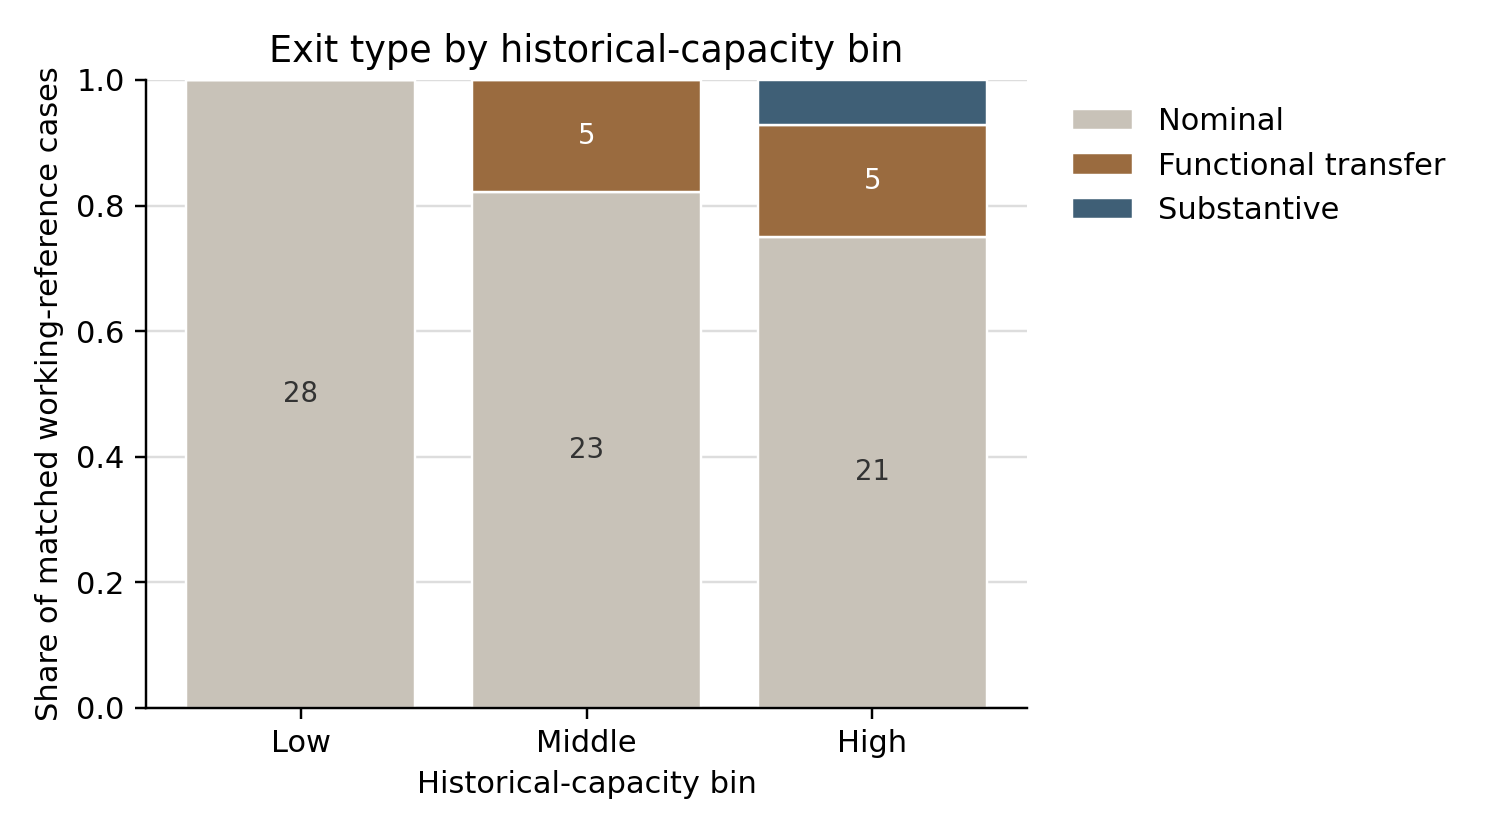
\includegraphics[width=0.82\linewidth]{figures/pilot_exit_type_by_capacity_bin.png}
\caption{Exit type by historical-capacity bin}
\label{fig:pilot-exit-type-by-capacity-bin}
\end{figure}

The case evidence clarifies the distinctions. Guangzhou City Construction
Investment and Ningbo Development Investment receive substantive-exit labels
because the reviewed packets indicate movement away from off-budget
government-project financing. Guangzhou's former government project work is
described as fiscally funded entrusted management rather than financing by the
platform. Xuzhou, Yancheng, and Hengyang receive nominal-exit labels because
formal exit or no-government-financing language coexists with infrastructure
construction, land preparation, government settlement, fiscal support,
repayment exposure, or entrusted construction. Hangzhou and Wenzhou illustrate
functional transfer: the public function remains in a reorganized municipal
state-owned system even though its issuer or organizational location changes.

These contrasts do not imply that historical capacity determines fate. The
reference set contains many high-capacity nominal exits. They show that strong
administrative inheritance can coexist with continuing platform finance when
development-zone mandates, debt pressure, land dependence, or local investment
commitments preserve the demand for an off-budget organization.

\subsection{Exploratory historical association}

The statistical application defines institutional change as substantive exit or
functional transfer, with nominal exit as zero. This binary outcome does not
collapse the conceptual distinction between absorption and transfer. It
provides a feasible exploratory comparison because the matched sample contains
only two substantive exits and no liquidation.

% Publication-facing rendering of EXP-20260830-012.
\begin{table}[htbp]
\centering
\caption{Exploratory sparse-outcome audit of historical capacity}
\label{tab:exploratory-sparse-outcome-audit}
\small
\setlength{\tabcolsep}{4pt}
\begin{tabular}{@{}lcccc@{}}
\toprule
 & Hist. LPM & Hist. Firth & Adj. LPM & Adj. Firth \\
\midrule
Elite-density effect & 0.066 & 0.056 & 0.005 & 0.003 \\
 & (0.041) & (0.032) & (0.045) & (0.052) \\
\midrule
Observations & 84 & 84 & 78 & 78 \\
Institutional-change events & 12 & 12 & 12 & 12 \\
Contemporary controls & No & No & Yes & Yes \\
Province fixed effects & No & No & No & No \\
\bottomrule
\end{tabular}
\begin{minipage}{0.94\linewidth}
\vspace{0.5em}\footnotesize Notes: This table is an exploratory diagnostic, not
a causal estimate. The outcome equals one for substantive exit or functional
transfer and zero for nominal exit. Effects are probability-point changes for
a one-sample-standard-deviation increase in elite density. LPM uncertainty is
HC1. Firth effects are average marginal effects with curvature-based
delta-method uncertainty shown only as a diagnostic. Adjusted models use
district-and-county platforms as the reference category. All fixed models were
reported without selection by sign or statistical significance.
\end{minipage}
\end{table}


Table~\ref{tab:exploratory-sparse-outcome-audit} reports the full fixed set of
historical-only and adjusted specifications. In the 84 matched cases, a
one-standard-deviation increase in historical elite density is associated with
a 6.6 percentage point increase in institutional change in the linear
probability model and a 5.6 percentage point average marginal effect in the
Firth logit. Their respective 95 percent diagnostic intervals are
$[-1.3,14.6]$ and $[-0.8,11.9]$ percentage points; both include zero.
Appendix Table~\ref{tab:pilot-lpm-institutional-change} retains the alternative
high-capacity and ordered-bin comparisons. The estimates describe the
assembled cases rather than a national probability sample. Elite density may
also capture persistent education or social capital.

The adjusted results are less stable. Contemporary controls are available for
78 of the 84 matched cases. Complete-case restriction removes six low-capacity
nominal exits while retaining all twelve institutional-change events. A
preregistered audit repairs the former rank deficiency by using
district-and-county platforms as the reference category. The corrected design
has eight independent columns and twelve events, or 1.5 events per column. The
adjusted linear probability and Firth-logit effects are 0.5 and 0.3 percentage
points. Deleting one observation at a time changes their signs in nine and
eleven of 78 fits, respectively. The two historical-only effects change sign
in zero deletions. Province fixed effects are not estimated because
only four of eighteen provinces have within-province outcome variation and the
candidate design would contain 25 columns for twelve events. Contemporary
fiscal capacity, debt pressure, land-finance dependence,
province, disclosure quality, platform level, and capital or sub-provincial
status remain alternative explanations rather than established controls for a
causal historical effect.

\subsection{LLM screening and the validation boundary}

The LLM-assisted file expands documentary screening without expanding the set
of final outcomes. Among 361 candidate disclosure rows, 346 have usable source
text or a reviewed status. The exit-type portion contains the 94 reference
labels and 203 one-sided nominal-exit surrogates. Forty-four reviewed packets
lack a directly documented formal event, five are boundary packets, and fifteen
lack a usable source packet.

% Auto-generated by scripts/build_llm_screening_sample.py
\begin{table}[htbp]
\centering
\caption{LLM screening status for the candidate pool}
\label{tab:llm-screening-status}
\small
\begin{tabular}{@{}lrr@{}}
\toprule
Screening status & Rows & Use \\
\midrule
Working reference label & 94 & Provisional documentary outcome \\
LLM surrogate exit type & 203 & One-sided provisional nominal screen \\
LLM screened, no direct formal event & 44 & Screened non-outcome \\
Source-packet-reviewed boundary & 5 & Scope condition \\
Source packet missing & 15 & Not usable \\
\midrule
Usable LLM screening rows & 346 & Screening sample \\
Usable exit-type rows & 297 & Outcome sample \\
\bottomrule
\end{tabular}
\begin{minipage}{0.94\linewidth}
\vspace{0.5em}\footnotesize Notes: A usable screening row has a working reference label, an LLM surrogate label, a source-packet-reviewed boundary decision, or source text screened as lacking a direct formal event. Working reference labels await independent human confirmation. Surrogate rows are not final four-category outcomes. Rows without a codable formal event are not assigned substantive, nominal, functional-transfer, or liquidation labels.
\end{minipage}
\end{table}


Repeated disclosures reduce the 203 surrogate rows to 158 issuers. Sixty-one
issuers also appear in the reference file; 97 do not. The 61 overlapping
issuers receive nominal labels under both procedures. This exact agreement
shows that the narrow screen can recover a documentary pattern already
recognized by the codebook. It is not probability-sample precision. The
overlap was formed after positive screening, and no screen-negative issuer has
a working-reference label. The data therefore do not identify recall,
four-category calibration, or error among screen-negative cases.

Table~\ref{tab:validation-identification-bounds} quantifies what the missing
labels permit without assuming that the observed overlap represents the other
issuers. If $K_+$ reference outcomes establish membership in a class, $K_-$
establish nonmembership, and $U$ are unknown, the finite-screen share lies
between $K_+/N$ and $(K_++U)/N$. For the 158 screen-positive issuers, the
conditional bounds are 38.61 to 100 percent. This wide range is compatible
with the selected 61-of-61 concordance because 97 issuer outcomes remain
unknown.

These bounds require the linked reference labels to be correct and applicable
to the corresponding issuer and event. Shared source documents are found for
41 links, but issuer matching and documentary overlap do not establish
independent same-event pairing. Without the applicability assumption, the
unconditional bounds are zero to 100 percent. The table therefore reports
identified sets conditional on stated evidence, not accuracy confidence
intervals, and it does not turn excluded or no-event cases into negative
outcomes.

% Generated by scripts/build_validation_identification_bounds.py; EXP-20260910-006
\begin{table}[htbp]
\centering
\small
\caption{Conditional finite-screen identification bounds}
\label{tab:validation-identification-bounds}
\setlength{\tabcolsep}{3pt}
\begin{tabular}{@{}lrrrrrr@{}}
\toprule
Population and quantity & $N$ & $K_+$ & $K_-$ & $U$ & Lower & Upper \\
\midrule
Screen: nominal membership & 158 & 61 & 0 & 97 & 38.61\% & 100.00\% \\
Screen: positive-label correctness & 158 & 61 & 0 & 97 & 38.61\% & 100.00\% \\
Screen: no reference overlap & 97 & 0 & 0 & 97 & 0.00\% & 100.00\% \\
Candidate: nominal membership & 67 & 0 & 0 & 67 & 0.00\% & 100.00\% \\
Candidate: positive-label correctness & 57 & 0 & 0 & 57 & 0.00\% & 100.00\% \\
Candidate: no direct event & 10 & 0 & 0 & 10 & 0.00\% & 100.00\% \\
\bottomrule
\end{tabular}
\par\vspace{4pt}
\begin{minipage}{\linewidth}\footnotesize
Notes: $K_+$ and $K_-$ count retained reference labels establishing membership and nonmembership;
$U=N-K_+-K_-$ counts unknown outcomes. The bounds are $K_+/N$ and $(K_++U)/N$.
Selected post-hoc overlap concordance is 61/61, reported separately.
The author report covers 94 unchanged reference labels, not candidate outcomes.
All bounds condition on each linked reference outcome being valid for the corresponding screen issuer/event.
Issuer matching does not prove event/time alignment or independent same-event pairing.
No sampling or missingness model is imposed;
these are neither confidence intervals nor performance-validation estimates. Scope exclusions and
no-direct-event flags are not coded as negative outcomes. The finite issuer screen is not a population
of verified eligible exits, and the candidate remains a proposal pending final freeze and human coding.
\end{minipage}
\end{table}


The source-verified 67-unit validation frame described in the previous section
addresses geographic and platform-scope coverage, but it is distinct from the
94-case human-checked reference file. The case-matching audit finds no exact
issuer/event match to that report, and the new collection sheets contain no
human decisions. Its proposed census weights cannot be
attached retrospectively to the selected 61-issuer overlap. A validation-adjusted
estimate requires observed human outcomes from the specified frame and a
record of their actual selection and response status. The following subsection
specifies the estimator and distinguishes this requirement from code execution.

\subsection{Design-based estimation}

The next analysis distinguishes the sampling design from the outcome model.
The residual correction in design-based supervised learning combines predictions
with observed human labels and their known selection probabilities
\citep{egami2023dsl}. I implement a finite-frame special case with predictions
fixed before validation selection. This form permits an exact check of the
estimator under the declared sampling design; it does not claim to implement
every learned or cross-fitted version of DSL.

Let $F$ contain $N$ admissible city-platform cases, let $Y_i$ be the declared
binary outcome, and let $m_i$ be its fixed auxiliary prediction. Let $R_i$
indicate selection for human labeling, with known probability $\pi_i>0$.
With complete responses from the selected cases, define
\begin{equation}
\widehat\mu_F=\frac{1}{N}\left\{
\sum_{i\in F}m_i+
\sum_{i\in F:R_i=1}\frac{Y_i-m_i}{\pi_i}\right\}.
\label{eq:validation-mean}
\end{equation}
The first term uses predictions for every case and the second corrects their
errors using the human-labeled sample. Because the design expectation of
$R_i/\pi_i$ is one, the expected correction recovers the frame mean even when
the fixed predictions are inaccurate. This statement concerns selection within
$F$, not representative sampling of LGFVs from China.

For independent simple random sampling without replacement within strata,
let $N_h$ and $n_h$ denote the stratum population and sample sizes. With
$e_i=Y_i-m_i$ and its sample variance $s^2_{e,h}$, the design variance estimator is
\begin{equation}
\widehat V(\widehat\mu_F)=
\sum_h\left(\frac{N_h}{N}\right)^2
\left(1-\frac{n_h}{N_h}\right)\frac{s^2_{e,h}}{n_h}.
\label{eq:validation-variance}
\end{equation}
A noncensus stratum with only one observed case does not identify its residual
variance. Each census stratum contributes zero to the variance by design,
including a singleton for which $s^2_{e,h}$ is undefined. A completed census
sets $R_i=\pi_i=1$ for every unit, so
Equation~\ref{eq:validation-mean} reduces to the observed human-label mean.
Its label-selection variance is zero, but coding uncertainty and uncertainty
about a broader population remain. No efficiency gain from surrogate labels
is claimed for that census.

The same correction can be used for the finite-frame linear projection when
the covariates $X_i$ are observed throughout the declared analytical frame:
\begin{equation}
\widehat\beta_F=
\left(\sum_{i\in F}X_iX_i^{\prime}\right)^{-1}
\left\{\sum_{i\in F}X_im_i+
\sum_{i\in F:R_i=1}\frac{X_i(Y_i-m_i)}{\pi_i}\right\}.
\label{eq:validation-projection}
\end{equation}
This is an associational summary with a fixed, full-rank design matrix.
Missing controls, post-selection response loss, and undefined exit outcomes
cannot be repaired by inserting the proposed sampling weights. In particular,
failure to find a formal event does not supply a zero for the
institutional-change outcome. The implemented checks therefore distinguish proposed weights,
actual selection, completed human decisions, and analytical eligibility before
releasing a numerical result. The estimates reported above remain
reference-sample analyses rather than completed validation-adjusted estimates.

\subsection{Contemporary process evidence}

The source packets contain evidence consistent with three contemporary
processes. Fiscal absorption is visible when former platform functions move
into budgetary channels, special-purpose bonds, or fiscally funded project
management. Bureaucratic coordination is visible in documented asset
transfers, debt succession, municipal platform-group reorganization, and
cross-agency implementation. Project and state-asset governance is visible
when the post-exit arrangement clarifies project preparation, repayment
responsibility, fiscal settlement, and the boundary between state-owned
enterprise activity and implicit government financing.

Appendix Table \ref{tab:pilot-mechanism-evidence} records these documentary
indicators. Substantive-exit packets tend to show absorption into formal fiscal
channels or unusually strong negative evidence of continued platform
financing. Functional-transfer packets show reorganization while preserving a
public function inside the local state-owned system. Nominal-exit packets retain
public-project, repayment, land-development, entrusted-construction, or fiscal
support functions inside the same issuer. These patterns make the theoretical
processes observable, but they do not identify mediation from historical elite
density to contemporary exit fate. Fiscal resources, coordinated compliance,
political connections, and other forms of institutional persistence remain
plausible alternatives.

\section{Conclusion}

Official exit is not institutional exit. A local government financing vehicle
may leave a regulatory list or adopt no-government-financing language while the
same public-finance function remains with the issuer, moves to another
state-owned entity, enters formal fiscal channels, or disappears with the legal
entity. This paper makes that institutional fate measurable by pairing a
documented formal event with evidence about the post-event location of the
function and assigning one of four mutually exclusive labels.

The measurement framework is the paper's main contribution. The current
working-reference file contains 94 Codex source-packet-reviewed cases awaiting
independent human confirmation, each linked to an event,
function evidence, an alternative label, and quality scores. All evidence
identifiers resolve to the source inventory, 93 cases have complete local
copies, and all 94 have recovery URLs. These features make each decision
auditable. They do not substitute for independent human validation: no human
reviewer has yet frozen confirmation decisions, and the current cases were not drawn from a
national probability frame.

The LLM screen serves the same measurement goal at a larger scale. It finds
one-sided nominal-exit candidates in repeated bond disclosures, but it does not
supply final four-category outcomes. The 61 issuers shared by the screen and
reference set agree exactly, yet that selected overlap cannot identify
population precision, recall, or multiclass error. Design-based supervised
learning can support validation-adjusted inference only after the project
verifies the issuer frame, draws cases with known probabilities, and obtains
independent human labels.

The historical application is therefore evidence about how the measure can be
used, not the paper's settled causal result. Among 84 matched reference cases,
historical elite density is positively associated with movement away from
nominal exit in simple models. The adjusted association is fragile under
complete-case restriction and case deletion, and the proxy may capture
education or social capital as well as administrative development.
Documentary patterns are consistent with fiscal absorption, bureaucratic
coordination, and project or state-asset governance, but the current design
does not identify those processes as mediators.

The resulting contribution is narrower and more durable than an official exit
count. It provides a source-auditable way to distinguish formal compliance from
functional fiscal change and shows why that distinction matters for the study
of central mandates, local adaptation, and quasi-fiscal organizations. A
submission-ready causal application will require a verified probability frame,
an independent second-coder round, broader representation of rare institutional
fates, and stable contemporary controls. Those additions extend the measure;
they do not change the institutional distinction on which the paper is built.


\appendix
\section{Working Reference Evidence Appendix}

This appendix reports the case-level evidence behind the validated empirical
section. The tables are intentionally detailed. The main text uses summary
patterns, while the appendix lets readers inspect how each label, historical
capacity match, and mechanism claim is supported by source material.

\subsection{Validated Labels}

Table \ref{tab:pilot-validated-labels} reports the working reference labels in
the historically matched subset. The table records the event basis for
each label, the final exit type, and the matched historical elite-density
measure. It is the case-level counterpart to the summary counts in the main
text.

% Auto-generated by scripts/build_pilot_capacity_summary.py
\begin{table}[htbp]
\centering
\caption{Human-validated pilot labels}
\label{tab:pilot-validated-labels}
\small
\begin{tabular}{@{}>{\raggedright\arraybackslash}p{0.13\linewidth}>{\raggedright\arraybackslash}p{0.42\linewidth}>{\raggedright\arraybackslash}p{0.19\linewidth}r@{}}
\toprule
City & Event basis & Final label & Elite density \\
\midrule
Guangzhou & 2014 fiscal-funded project management & Substantive exit & 212.95 \\
Hangzhou & 2022 municipal platform consolidation & Functional transfer & 158.93 \\
Chengdu & 2015 no-government-financing language & Nominal exit & 79.18 \\
Xi'an & 2012 platform-list exit disclosure & Nominal exit & 52.58 \\
Zhuzhou & 2013 banking-regulator platform-list exit & Nominal exit & 9.19 \\
\bottomrule
\end{tabular}
\begin{minipage}{0.96\linewidth}
\vspace{0.5em}\footnotesize Notes: Final labels are assigned after human review of the original source packets and are not assigned to source-only candidates. Elite density is measured as Ming-Qing jinshi and juren records per 1,000 square kilometers in the matched contemporary prefecture.
\end{minipage}
\end{table}


\subsection{Historical Capacity Matches}

Table \ref{tab:pilot-historical-capacity} reports the CBDB-GADM
historical-capacity match used in the empirical analysis. The table includes the
eighty-four historically matched working reference cases and three candidate cases retained
for comparison or future source collection.

% Auto-generated by scripts/build_pilot_capacity_summary.py
\begingroup
\small
\begin{longtable}{lllr}
\caption{Validated cases and historical elite density}\label{tab:pilot-historical-capacity}\\
\toprule
City & Case status & Exit type/status & Elite density \\
\midrule
\endfirsthead
\toprule
City & Case status & Exit type/status & Elite density \\
\midrule
\endhead
Jiaxing & Working reference & Nominal exit & 461.93 \\
Jiaxing & Working reference & Nominal exit & 461.93 \\
Suzhou & Working reference & Nominal exit & 314.34 \\
Suzhou & Working reference & Functional transfer & 314.34 \\
Suzhou & Working reference & Nominal exit & 314.34 \\
Suzhou & Working reference & Nominal exit & 314.34 \\
Suzhou & Working reference & Nominal exit & 314.34 \\
Changzhou & Working reference & Nominal exit & 314.13 \\
Changzhou & Working reference & Nominal exit & 314.13 \\
Changzhou & Working reference & Nominal exit & 314.13 \\
Fuzhou & Working reference & Functional transfer & 218.49 \\
Fuzhou & Working reference & Functional transfer & 218.49 \\
Guangzhou & Working reference & Substantive exit & 212.95 \\
Guangzhou & Working reference & Nominal exit & 212.95 \\
Guangzhou & Working reference & Nominal exit & 212.95 \\
Wuxi & Working reference & Functional transfer & 207.55 \\
Ningbo & Working reference & Substantive exit & 196.82 \\
Ningbo & Working reference & Nominal exit & 196.82 \\
Shaoxing & Working reference & Nominal exit & 188.01 \\
Huzhou & Working reference & Nominal exit & 170.05 \\
Hangzhou & Working reference & Functional transfer & 158.93 \\
Beijing & Working reference & Nominal exit & 136.30 \\
Zhenjiang & Working reference & Nominal exit & 133.11 \\
Jinan & Working reference & Nominal exit & 116.10 \\
Jinan & Working reference & Nominal exit & 116.10 \\
Jinan & Working reference & Nominal exit & 116.10 \\
Nanjing & Working reference & Nominal exit & 101.55 \\
Nanjing & Working reference & Nominal exit & 101.55 \\
Nanjing & Working reference & Nominal exit & 101.55 \\
Nanjing & Working reference & Nominal exit & 101.55 \\
Nanjing & Working reference & Nominal exit & 101.55 \\
Foshan & Working reference & Functional transfer & 100.72 \\
Chengdu & Working reference & Nominal exit & 79.18 \\
Tianjin & Working reference & Nominal exit & 76.32 \\
Tianjin & Working reference & Nominal exit & 76.32 \\
Fuzhou & Working reference & Nominal exit & 66.49 \\
Ji'an & Working reference & Nominal exit & 60.86 \\
Xi'an & Working reference & Nominal exit & 52.58 \\
Taizhou & Working reference & Functional transfer & 49.99 \\
Taizhou & Working reference & Nominal exit & 49.99 \\
Taizhou & Working reference & Nominal exit & 49.99 \\
Xuchang & Working reference & Nominal exit & 46.00 \\
Shangrao & Working reference & Nominal exit & 45.86 \\
Shangrao & Working reference & Nominal exit & 45.86 \\
Xiaogan & Working reference & Functional transfer & 45.71 \\
Dezhou & Working reference & Nominal exit & 38.11 \\
Taizhou & Working reference & Functional transfer & 36.81 \\
Jingdezhen & Working reference & Nominal exit & 36.46 \\
Wenzhou & Working reference & Functional transfer & 30.20 \\
Huai'an & Working reference & Nominal exit & 30.12 \\
Zhengzhou & Working reference & Nominal exit & 29.77 \\
Jinzhong & Working reference & Nominal exit & 26.19 \\
Shijiazhuang & Working reference & Nominal exit & 25.05 \\
Xingtai & Working reference & Nominal exit & 24.14 \\
Luoyang & Working reference & Nominal exit & 22.14 \\
Kunming & Working reference & Nominal exit & 20.74 \\
Huangshi & Working reference & Nominal exit & 19.39 \\
Huangshi & Working reference & Nominal exit & 19.39 \\
Hengyang & Working reference & Nominal exit & 18.58 \\
Jingmen & Working reference & Nominal exit & 18.19 \\
Qingdao & Working reference & Nominal exit & 18.12 \\
Qingdao & Working reference & Nominal exit & 18.12 \\
Rizhao & Working reference & Nominal exit & 17.62 \\
Linyi & Working reference & Nominal exit & 12.48 \\
Luzhou & Working reference & Nominal exit & 11.36 \\
Luzhou & Strong candidate & Near-miss functional persistence & 11.36 \\
Ganzhou & Working reference & Nominal exit & 10.48 \\
Zhuzhou & Working reference & Nominal exit & 9.19 \\
Lu'an & Working reference & Nominal exit & 8.64 \\
Bengbu & Working reference & Nominal exit & 8.13 \\
Nantong & Working reference & Nominal exit & 7.52 \\
Nantong & Working reference & Nominal exit & 7.52 \\
Nantong & Working reference & Nominal exit & 7.52 \\
Zunyi & Weak-capacity candidate & Source started & 7.21 \\
Suzhou & Working reference & Nominal exit & 6.80 \\
Yiyang & Working reference & Nominal exit & 6.56 \\
Leshan & Working reference & Nominal exit & 6.24 \\
Xuzhou & Working reference & Nominal exit & 5.52 \\
Xuzhou & Working reference & Nominal exit & 5.52 \\
Xuzhou & Working reference & Nominal exit & 5.52 \\
Nanning & Working reference & Nominal exit & 3.61 \\
Bozhou & Working reference & Nominal exit & 2.33 \\
Bozhou & Working reference & Nominal exit & 2.33 \\
Yancheng & Working reference & Nominal exit & 2.21 \\
Yancheng & Working reference & Nominal exit & 2.21 \\
Liupanshui & Weak-capacity candidate & Documents found & 0.60 \\
Harbin & Working reference & Nominal exit & 0.02 \\
\bottomrule
\end{longtable}
\begin{minipage}{0.92\linewidth}
\vspace{0.5em}\footnotesize Notes: Elite density is the number of Ming-Qing jinshi and juren records matched from CBDB to GADM 4.1 China ADM2 boundaries, scaled per 1,000 square kilometers. Luzhou is a strong near-miss candidate rather than a final working-reference label because a direct platform-list exit source has not yet been found. Zunyi and Liupanshui are weak-capacity candidate cases rather than working-reference exit-type cases.
\end{minipage}
\endgroup


\subsection{Alternative historical comparisons}

Table~\ref{tab:pilot-lpm-institutional-change} retains the historical-density,
high-capacity, and ordered-bin comparisons. The main text reports the fixed
historical-only and adjusted linear probability and Firth specifications
together so that the unstable adjusted result is not separated from the
unadjusted association.

% Auto-generated by scripts/build_pilot_empirical_models.py
\begin{table}[htbp]
\centering
\caption{Exploratory pilot association between historical capacity and institutional change}
\label{tab:pilot-lpm-institutional-change}
\small
\setlength{\tabcolsep}{4pt}
\begin{tabular}{@{}lccc@{}}
\toprule
 & (1) & (2) & (3) \\
 & Institutional change & Institutional change & Institutional change \\
\midrule
Elite density, standardized & 0.120* &  &  \\
 & (0.066) &  &  \\
High historical-capacity bin &  & 0.225* &  \\
 &  & (0.121) &  \\
Capacity bin rank &  &  & 0.175*** \\
 &  &  & (0.054) \\
Intercept & 0.200*** & 0.125** & 0.025 \\
 & (0.050) & (0.053) & (0.038) \\
\midrule
Observations & 60 & 60 & 60 \\
Mean of dependent variable & 0.200 & 0.200 & 0.200 \\
\bottomrule
\end{tabular}
\begin{minipage}{0.94\linewidth}
\vspace{0.5em}\footnotesize Notes: The dependent variable equals one for substantive exit or functional transfer and zero for nominal exit. The table uses the sixty human-validated cases currently matched to the CBDB-GADM historical-capacity measure. Coefficients are linear probability models with HC1 robust standard errors in parentheses. These estimates are exploratory pilot associations rather than population or causal estimates. $^{*}p<0.10$, $^{**}p<0.05$, $^{***}p<0.01$.
\end{minipage}
\end{table}


\subsection{Disclosure and issuer counts}

The disclosure-to-issuer construction retains repeated source packets and
separates observed reference outcomes from unvalidated surrogate outputs.
Its combined rows are not a probability validation sample.

% Auto-generated by scripts/build_surrogate_empirical_core.py
\begin{table}[htbp]
\centering
\caption{From disclosure screening to issuer-level empirical inputs}
\label{tab:surrogate-empirical-flow}
\small
\setlength{\tabcolsep}{4pt}
\begin{tabular}{@{}p{0.43\linewidth}rp{0.36\linewidth}@{}}
\toprule
Step & Count & Role \\
\midrule
Candidate disclosure rows & 361 & Initial source-packet pool \\
Usable LLM screening rows & 346 & Rows with source text or validated status \\
Exit-type rows & 297 & Reference labels plus provisional surrogate labels \\
LLM surrogate disclosure labels & 203 & Medium-confidence nominal-exit screens \\
Issuer-level surrogate rows & 158 & Deduplicated auxiliary labels \\
Surrogate issuers overlapping reference labels & 61 & Selected-overlap consistency check \\
Non-overlap surrogate issuers & 97 & Awaiting probability-frame validation \\
Reference plus non-overlap issuer rows & 191 & Descriptive construction only \\
Screened rows without direct formal event & 44 & Screening attrition, not exit-type outcomes \\
Source-packet missing rows & 15 & Not used \\
\bottomrule
\end{tabular}
\begin{minipage}{0.94\linewidth}
\vspace{0.5em}\footnotesize Notes: Disclosure-level rows are source packets, while issuer-level rows deduplicate repeated bond disclosures for the same issuer. The 61 overlaps were formed after positive screening and therefore do not estimate population precision or recall. The 191-row construction is not used as a validation-adjusted outcome sample.
\end{minipage}
\end{table}


\subsection{Mechanism Evidence}

Table \ref{tab:pilot-mechanism-evidence} reports qualitative mechanism notes
for the historically matched working reference cases. These notes are not treated as
separate quantitative outcomes. Their role is to show whether the
documentary record contains evidence relevant to fiscal absorption,
bureaucratic coordination, and project or state-asset governance.

% Auto-generated by scripts/build_pilot_capacity_summary.py
\begin{table}[p]
\centering
\caption{Mechanism evidence in human-validated pilot cases}
\label{tab:pilot-mechanism-evidence}
\begingroup
\scriptsize
\renewcommand{\arraystretch}{0.92}
\setlength{\tabcolsep}{2pt}
\begin{tabular}{@{}>{\raggedright\arraybackslash}p{0.10\linewidth}>{\raggedright\arraybackslash}p{0.12\linewidth}>{\raggedright\arraybackslash}p{0.23\linewidth}>{\raggedright\arraybackslash}p{0.25\linewidth}>{\raggedright\arraybackslash}p{0.25\linewidth}@{}}
\toprule
City & Label & Fiscal absorption & Bureaucratic coordination & Project and asset governance \\
\midrule
Guangzhou & Substantive exit & Budget-funded project management and 2018 fiscal debt replacement. & Post-2014 role shift appears across issuer, rating, and debt-replacement documents. & Public projects remain as management tasks rather than new platform financing. \\
Ningbo & Substantive exit & Negative evidence shows no government purchase service, BT, PPP, land preparation, or fiscal repayment. & Issuer-level compliance evidence is strong; an independent list source is still missing. & No major continuing platform function is found; a residual receivable is treated as engineering background. \\
Hangzhou & Functional transfer & Debt succession and asset transfer occurred through formal reorganization. & Qiantou transfer, city-investment consolidation, and Anju creation link multiple municipal entities. & Public project and housing functions moved within the municipal platform system. \\
Jinan & Nominal exit & Land-preparation gains and fiscal subsidies compensate the issuer. & Non-platform-list disclosure is present; the original list basis has not yet been collected. & Land preparation, government authorization, infrastructure, affordable housing, and entrusted assets continue. \\
Foshan & Functional transfer & Fiscal settlement for entrusted construction and contract-based payments are documented. & SASAC-entrusted land preparation coexists with disclosure that the issuer was outside the 2018 platform directory. & Public project tasks are formalized through SASAC-owned land and contract settlement. \\
Chengdu & Nominal exit & Debt replacement and government-bond pass-through coexist with fiscal-payment chains. & Issuer compliance language is present, but an independent exit-list source is still missing. & The same issuer continues infrastructure investment and financing functions. \\
Xi'an & Nominal exit & Direct fiscal-substitution evidence remains limited. & The 2012 platform-list exit is issuer-disclosed; later business-module transfers appear partial. & The issuer retains BT, entrusted-construction, and government-repurchase exposure. \\
Wenzhou & Functional transfer & Fiscal construction payments and fiscal compensation remain visible. & Issuer-level compliance is paired with group-level relocation of public functions. & The municipal group continues land preparation, affordable housing, and public-utility functions. \\
Hengyang & Nominal exit & Annual government payments for entrusted construction and fiscal subsidies remain visible. & Exit, re-entry, and 2020 CBIRC transfer-out language give the formal event unusual clarity. & The same issuer continues entrusted construction, land preparation, infrastructure, and affordable housing. \\
Zhuzhou & Nominal exit & Service-contract and fiscal-settlement evidence appears after formal exit. & Hunan banking-regulator exit is reported in issuer and legal documents. & Land preparation, major projects, fiscal settlement, and government support continue. \\
Xuzhou & Nominal exit & Budgeted government-purchase payments, fiscal subsidies, and project-repurchase support remain visible. & Issuer no-government-financing language is present; a direct government list source is still missing. & Shantytown redevelopment, water infrastructure, land preparation, and entrusted construction continue. \\
Yancheng & Nominal exit & Government-supported affordable housing and real-business-background government receivables remain visible. & Issuer compliance language is present; a separate platform-list source is still missing. & Land preparation, infrastructure entrusted construction, and affordable housing continue. \\
\bottomrule
\end{tabular}
\endgroup
\end{table}


\subsection{Source Audit}

Table \ref{tab:pilot-source-audit} records the source trail behind the
historically matched working reference labels. The full human-checked reference file now
contains ninety-four cases, and this table reports the eighty-four cases currently
matched to the CBDB-GADM historical-capacity crosswalk. For each case, it
lists the primary document used for the label, the formal exit or compliance event, the observed
post-event function, and the final coding decision. The table is deliberately
redundant with the case packets. Its purpose is to let readers see where the
coding judgment comes from before accepting the descriptive patterns in the
main empirical section.

% Auto-generated by scripts/build_pilot_capacity_summary.py
\begin{table}[p]
\centering
\caption{Source audit for historically matched pilot labels}
\label{tab:pilot-source-audit}
\begingroup
\tiny
\renewcommand{\arraystretch}{0.92}
\setlength{\tabcolsep}{2pt}
\begin{tabular}{@{}>{\raggedright\arraybackslash}p{0.10\linewidth}>{\raggedright\arraybackslash}p{0.17\linewidth}>{\raggedright\arraybackslash}p{0.23\linewidth}>{\raggedright\arraybackslash}p{0.34\linewidth}>{\raggedright\arraybackslash}p{0.10\linewidth}@{}}
\toprule
City & Primary source & Formal event & Post-event function & Label \\
\midrule
Guangzhou & 2026 MTN disclosure, lines 927-931;6537-6548;6756-6761 & 2014 shift away from new government-project investment-financing & budget-funded project management and city construction functions remained & Substantive exit \\
Ningbo & 2026 prospectus, lines 927-932 & 2015 no-government-financing language and explicit absence of core platform businesses & No major continuing platform function found in the prospectus; residual engineering receivable disclosed as non-financing background & Substantive exit \\
Hangzhou & 2024 prospectus, lines 1188-1192;222-228;272-288 & 2022 reorganization through Qiantou equity transfer and Anju creation & public project and debt functions continued inside enlarged city investment system & Functional transfer \\
Jinan & 2025 prospectus, lines 1193-1199;4572-4573 & 2015 no-government-financing language and not in banking-regulator platform list & land preparation government authorization infrastructure affordable housing fiscal compensation and historical entrusted construction assets & Nominal exit \\
Foshan & 2025 prospectus, lines 5102-5105;5137-5140 & Not in CBIRC local financing platform directory as of 2018 & SASAC-entrusted land preparation and fiscally settled entrusted-construction projects & Functional transfer \\
Chengdu & 2023 prospectus, lines 1662-1670;4884-4892;4902-4916 & 2015 no-government-financing language & continued infrastructure investment financing and fiscal-payment chains & Nominal exit \\
Xi'an & 2026 MTN disclosure, lines 774-783;656-663;724-728 & 2012 issuer-disclosed platform-list exit & continued BT entrusted construction infrastructure and repurchase by management committee & Nominal exit \\
Wenzhou & 2026 prospectus, lines 1054-1055;3239-3242;5606-5608 & No-government-financing language and non-platform-list disclosure at issuer level & Municipal construction group continues land preparation entrusted construction affordable housing public utility and fiscal entrusted construction receivable functions & Functional transfer \\
Hengyang & 2026 prospectus, lines 3465-3472 & 2011 exit 2012 re-entry and 2020 formal transfer out of CBIRC platform management & entrusted construction project financing government settlement land preparation infrastructure affordable housing fiscal subsidy evidence & Nominal exit \\
Zhuzhou & 2026 SCP disclosure, lines 4558-4575;4656-4665;3888-3907;4488-4499;4677-4688 & explicit March 2013 exit from platform list & land preparation major project and fiscal-settlement functions continued & Nominal exit \\
Xuzhou & 2026 prospectus, lines 1395-1398 & 2015 no-government-financing language & shantytown redevelopment municipal water facilities land preparation government purchase service entrusted construction and fiscal subsidies & Nominal exit \\
Yancheng & 2025 prospectus, lines 928-929 & 2015 no-government-financing language & land preparation infrastructure entrusted construction and affordable housing work & Nominal exit \\
\bottomrule
\end{tabular}
\endgroup
\end{table}


\clearpage

\bibliographystyle{plainnat}
\bibliography{references}

\end{document}
